%!TEX TS-program = xelatex
\documentclass[12pt, a4paper, oneside]{extreport}

%%%%%%%%%% Програмный код %%%%%%%%%%
\usepackage{minted}
\usemintedstyle{borland}
% Включает подсветку команд в программах!
% Нужно, чтобы на компе стоял питон, надо поставить пакет Pygments, в котором он сделан, через pip.

% Для Windows: Жмём win+r, вводим cmd, жмём enter. Открывается консоль.
% Прописываем easy_install Pygments
% Заходим в настройки texmaker и там прописываем в PdfLatex:
% pdflatex -shell-escape -synctex=1 -interaction=nonstopmode %.tex

% Для Linux: Открываем консоль. Убеждаемся, что у вас установлен pip командой pip --version
% Если он не установлен, ставим его: sudo apt-get install python-pip
% Ставим пакет sudo pip install Pygments

% Для Mac: Всё то же самое, что на Linux, но через brew.

% После всего этого вы должны почувствовать себя тру-программистами!
% Документация по пакету хорошая. Сам читал, погуглите!




%%%%%%%%%% Математика %%%%%%%%%%
\usepackage{amsmath,amsfonts,amssymb,amsthm,mathtools}
\mathtoolsset{showonlyrefs=true}  % Показывать номера только у тех формул, на которые есть \eqref{} в тексте.
%\usepackage{leqno} % Нумерация формул слева



%%%%%%%%%%%%%%%%%%%%%%%% Шрифты %%%%%%%%%%%%%%%%%%%%%%%%%%%%%%%%%
\usepackage[english, russian]{babel} % выбор языка для документа
\usepackage[utf8]{inputenc} % задание utf8 кодировки исходного tex файла
\usepackage[X2,TS1, T2A]{fontenc}        % кодировка
\usepackage{cmap}


\usepackage{fontspec}         % пакет для подгрузки шрифтов
\setmainfont{Linux Libertine O}   % задаёт основной шрифт документа

% Шрифт для кода
\setmonofont[Scale=0.85]{Monaco}
\usepackage{verbments}

\usepackage{unicode-math}     % пакет для установки математического шрифта
\setmathfont[math-style=upright]{Neo Euler} % шрифт для математики

%%%%%%%%%% Работа с картинками %%%%%%%%%
\usepackage{graphicx}                  % Для вставки рисунков
\usepackage{graphics}
\graphicspath{{images/}{pictures/}}    % можно указать папки с картинками
\usepackage{wrapfig}                   % Обтекание рисунков и таблиц текстом


%%%%%%%%%% Работа с таблицами %%%%%%%%%%
\usepackage{tabularx}            % новые типы колонок
\usepackage{tabulary}            % и ещё новые типы колонок
\usepackage{array}               % Дополнительная работа с таблицами
\usepackage{longtable}           % Длинные таблицы
\usepackage{multirow}            % Слияние строк в таблице
\usepackage{float}               % возможность позиционировать объекты в нужном месте
\usepackage{booktabs}            % таблицы как в книгах!
\renewcommand{\arraystretch}{1.3} % больше расстояние между строками

% Заповеди из документации к booktabs:
% 1. Будь проще! Глазам должно быть комфортно
% 2. Не используйте вертикальные линни
% 3. Не используйте двойные линии. Как правило, достаточно трёх горизонтальных линий
% 4. Единицы измерения - в шапку таблицы
% 5. Не сокращайте .1 вместо 0.1
% 6. Повторяющееся значение повторяйте, а не говорите "то же"
% 7. Есть сомнения? Выравнивай по левому краю!

%  вычисляемые колонки по tabularx
\newcolumntype{C}{>{\centering\arraybackslash}X}
\newcolumntype{L}{>{\raggedright\arraybackslash}X}
\newcolumntype{Y}{>{\arraybackslash}X}
\newcolumntype{Z}{>{\centering\arraybackslash}X}

% межстрочный отступ в таблице
\renewcommand{\arraystretch}{1.2}


%%%%%%%%%% Графика и рисование %%%%%%%%%%
\usepackage{tikz, pgfplots}  % язык для рисования графики из latex'a


%%%%%%%%%% Гиперссылки %%%%%%%%%%
\usepackage{xcolor}              % разные цвета

% Два способа включить в пакете какие-то опции:
%\usepackage[опции]{пакет}
%\usepackage[unicode,colorlinks=true,hyperindex,breaklinks]{hyperref}

\usepackage{hyperref}
\hypersetup{
	unicode=true,           % позволяет использовать юникодные символы
	colorlinks=true,       	% true - цветные ссылки, false - ссылки в рамках
	urlcolor=blue,          % цвет ссылки на url
	linkcolor=black,          % внутренние ссылки
	citecolor=black,        % на библиографию
	pdfnewwindow=true,      % при щелчке в pdf на ссылку откроется новый pdf
	breaklinks              % если ссылка не умещается в одну строку, разбивать ли ее на две части?
}

%%%%%%%%%% Другие приятные пакеты %%%%%%%%%
\usepackage{multicol}       % несколько колонок
\usepackage{verbatim}       % для многострочных комментариев
\usepackage{cmap}           % для кодировки шрифтов в pdf

% свешиваем пунктуацию
% теперь знаки пунктуации могут вылезать за правую границу текста, при этом текст выглядит ровнее
\usepackage{microtype}

\usepackage{enumitem} % дополнительные плюшки для списков
%  например \begin{enumerate}[resume] позволяет продолжить нумерацию в новом списке

\usepackage{todonotes} % для вставки в документ заметок о том, что осталось сделать
% \todo{Здесь надо коэффициенты исправить}
% \missingfigure{Здесь будет Последний день Помпеи}
% \listoftodos --- печатает все поставленные \todo'шки


%%%% Оформление %%%%%%%
% размер листа бумаги
\usepackage[
paperwidth=160mm,
paperheight=220mm,
headheight=14mm,
left=10mm,
right=10mm,
top=20mm,
bottom=20mm
]{geometry}

\usepackage{indentfirst}       % установка отступа в первом абзаце главы!!!

\usepackage{fancyhdr}

\pagestyle{fancy}
\fancyhf{}
\fancyhead[LE,RO]{\thepage}
\fancyhead[LO]{\leftmark}
\fancyhead[RE]{\rightmark}


\usepackage{setspace}
%\setstretch{1.3}  % Межстрочный интервал
%\setlength{\parindent}{1.5em} % Красная строка.
%\setlength{\parskip}{4mm}   % Расстояние между абзацами
% Разные длины в латехе https://en.wikibooks.org/wiki/LaTeX/Lengths

% \flushbottom                            % Эта команда заставляет LaTeX чуть растягивать строки, чтобы получить идеально прямоугольную страницу
\righthyphenmin=2                       % Разрешение переноса двух и более символов
\widowpenalty=300                     % Небольшое наказание за вдовствующую строку (одна строка абзаца на этой странице, остальное --- на следующей)
\clubpenalty=3000                     % Приличное наказание за сиротствующую строку (омерзительно висящая одинокая строка в начале страницы)
\tolerance=10000     % Ещё какое-то наказание.

\usepackage{bm}
\usepackage{bbm} % шрифт с двойными буквами

% свешиваем пунктуацию
% теперь знаки пунктуации могут вылезать за правую границу текста, при этом текст выглядит ровнее
\usepackage{microtype}

% для эпиграфов
\usepackage{epigraph} 
\setlength\epigraphrule{0pt}
\renewcommand{\textflush}{flushepinormal}

% Внешний вид подписей к картинкам и таблицам
\usepackage[font=small, labelfont=bf]{caption}
\DeclareCaptionLabelSeparator{colon}{\textbf{.} }
\DeclareCaptionLabelFormat{dash}{#1\hspace{.55ex}#2}
\captionsetup[figure]{labelformat=dash}




%%%%%%%%%% Свои команды %%%%%%%%%%
\usepackage{etoolbox}    % логические операторы для своих макросов

% Математические символы первой необходимости:
\DeclareMathOperator{\sgn}{sign}

\DeclareMathOperator*{\argmin}{arg\,min}
\DeclareMathOperator*{\argmax}{arg\,max}

\DeclareMathOperator{\Cov}{Cov}
\DeclareMathOperator{\Var}{Var}
\DeclareMathOperator{\Corr}{Corr}
\DeclareMathOperator{\E}{\mathop{E}}
\DeclareMathOperator{\Med}{Med}
\DeclareMathOperator{\Mod}{Mod}

\DeclareMathOperator*{\plim}{plim}

\newcommand{\const}{\mathrm{const}}        % const прямым начертанием

%% эконометрические сокращения
\def \hb{\hat{\beta}}
\def \hs{\hat{s}}
\def \hy{\hat{y}}
\def \hY{\hat{Y}}
\def \he{\hat{\varepsilon}}
\def \hVar{\widehat{\Var}}
\def \hCorr{\widehat{\Corr}}
\def \hCov{\widehat{\Cov}}

% Греческие буквы
\def \a{\alpha}
\def \b{\beta}
\def \t{\tau}
\def \dt{\delta}
\def \e{\varepsilon}
\def \ga{\gamma}
\def \kp{\varkappa}
\def \la{\lambda}
\def \sg{\sigma}
\def \tt{\theta}
\def \Dt{\Delta}
\def \La{\Lambda}
\def \Sg{\Sigma}
\def \Tt{\Theta}
\def \Om{\Omega}
\def \om{\omega}

% Готика
\def \mA{\mathcal{A}}
\def \mB{\mathcal{B}}
\def \mC{\mathcal{C}}
\def \mE{\mathcal{E}}
\def \mF{\mathcal{F}}
\def \mH{\mathcal{H}}
\def \mL{\mathcal{L}}
\def \mN{\mathcal{N}}
\def \mU{\mathcal{U}}
\def \mV{\mathcal{V}}
\def \mW{\mathcal{W}}

% Жирные штуки
\def \mbb{\mathbb}

\def \RR{\mbb R}
\def \NN{\mbb N}
\def \ZZ{\mbb Z}
\def \PP{\mbb{P}}
\def \QQ{\mbb Q}

% Карточные масти
\DeclareSymbolFont{extraup}{U}{zavm}{m}{n}
\DeclareMathSymbol{\varheart}{\mathalpha}{extraup}{86}
\DeclareMathSymbol{\vardiamond}{\mathalpha}{extraup}{87}


% Команды первой необходимости
\newcommand{\iid}{\mathrel{\stackrel{\rm i.\,i.\,d.}\sim}}  % ну вы поняли...
\newcommand{\fr}[2]{\ensuremath{^#1/_#2}}   % особая дробь
\newcommand{\ind}[1]{\mathbbm{1}_{\{#1\}}} % Индикатор события
\newcommand{\dx}[1]{\,\mathrm{d}#1} % для интеграла: маленький отступ и прямая d

\newcommand{\indef}[1]{\textbf{#1}}     % выделение ключевого слова в определениях

% бульпоинты в списках
\definecolor{myblue}{rgb}{0, 0.45, 0.70}
\newcommand*{\MyPoint}{\tikz \draw [baseline, fill=myblue,draw=blue] circle (2.5pt);}
\renewcommand{\labelitemi}{\MyPoint}

% для нормального распределения
\newcommand{\expp}[1]{ \exp \left( #1 \right)} 
% для прорисовки нормального распределения
\newcommand\gauss[2]{1/(#2*sqrt(2*pi))*exp(-((x-#1)^2)/(2*#2^2))} 



%%%%%%%%%% Теоремы %%%%%%%%%%
\theoremstyle{plain}              % Это стиль по умолчанию.  Есть другие стили.
\newtheorem{theorem}{Теорема}[section]
\newtheorem{result}{Следствие}[theorem]
% счётчик подчиняется теоремному, нумерация идёт по главам согласованно между собой


\theoremstyle{definition}         % убирает курсив и что-то еще наверное делает ;)
\newtheorem*{definition}{Определение}  % нумерация не идёт вообще

\newtheorem{chudo}{Чудо номер}   % Для первой главы



%%%%%%%%%% Список литературы %%%%%%%%%%

%\usepackage[backend=biber,style=chem-acs,sorting=nty]{biblatex}
% style --- стиль оформления библиографии
% backend --- Движок для сборки. Просто пишите сюда biber. Trust me.
% sorting --- Порядок сортировки в списке. nty = сначала по имени, потом по названию, потом по году выхода статьи. В этот же список можно включить 'a' - по алфавиту,


%\addbibresource{bayes.bib} % сюда нужно вписать свой биб-файлик


%%%%%%%%%% Задачи и их решения %%%%%%%%%%%

\usepackage{answers}

\newtheorem{problem}{\color{myblue} Упражнение}
\Newassociation{sol}{solution}{solution_file}
% sol --- имя окружения внутри задач
% solution --- имя окружения внутри solution_file
% solution_file --- имя файла в который будет идти запись решений
% можно изменить далее по ходу

\setlength{\epigraphwidth}{0.5\textwidth}

\usepackage{pgf,tikz}
\usepackage{mathrsfs}
\usetikzlibrary{arrows}

\begin{document}

% \Opensolutionfile{solution_file}[solutions1]

\chapter{Мама, папа, знакомьтесь, это STAN}

\epigraph{
	Варкалось. Хливкие шорьки \\
	Пырялись по наве, \\
	И хрюкотали зелюки, \\
	Как мюмзики в мове. \\
	\mbox{    }\\
	О, бойся Бармаглота, сын!\\
	Он так свирлеп и дик! \\
	А в глу́ши ры́мит исполин - \\
	Злопасный Брандашмыг...}{Льюис Кэрролл}

\section{Знакомство} 

Мы уже несколько раз говорили о том, что байесовский подход начал интенсивно развиваться в течение последних 30 лет. Прежде всего, это связано с  развитием компьютеров, которые позволили таскать за собой разные сложные распределения. В предыдущей главе мы с вами на простых примерах убедились, что расчёты  в байесовском мире делать не очень просто. Если взять в качестве априорного распределения что-то сложное, можно нарваться на проблемы.

 Из-за этого древние байесовцы поставили перед собой вполне разумную цель: брать в качестве априорных распределений такие, чтобы после домножения на правдоподобие апостериорное распределение принадлежало тому же классу распределений, но с другими параметрами. Эти новые параметры зависели бы от параметров априорного распределения, и наши алгоритмы бы просто осуществляли пересчёт априорных параметров в апостериорные по готовым формулам\footnote{На Википедии можно найти \href{https://en.wikipedia.org/wiki/Conjugate_prior}{огромную таблицу} с сопряжёнными распределениями}.  
 
 Это очень сильно связывало руки. Прошло время, и миру явился избранный\footnote{Слышишь гул мотора? Навуходоносор влетает в Зион.}.  Алгоритмы Монте-Карло по схеме Марковской цепи (MCMC) позволили разорвать оковы. Анализ моделей с априорными распределениями на любой вкус стал явью.
 
  Для генерации апостериорного распределения MCMC используются марковские цепи. По идее, при таком подходе от исследователя требуется сформулировать модель, априорное мнение о параметрах модели и самостоятельно сконструировать цепь, сходящуюся к апостериорному распределению параметров. Однако оказалось, что конструирование цепи в большинстве ситуаций можно доверить компьютеру. Это ещё сильнее упростило жизнь.
 
 В этой главе мы не будем разбираться в том, что именно происходит внутри чёрного ящика MCMC. Этому будут посвящены более поздние главы. Здесь мы на нескольких примерах посмотрим на то, как этот чёрный ящик можно применять в связке с R.
 
 Использовать для этого мы будем отличный, свободный, бесплатный, уютный вероятностный язык программирования STAN.  \href{http://mc-stan.org}{STAN} --- это не пакет R, а отдельный язык описания байесовских моделей. Исследователь описывает модель и априорное распределение параметров, а STAN генерирует код C++, в котором запрограммирована требуемая марковская цепь. %Среди альтернатив программе STAN можно назвать \href{http://mcmc-jags.sourceforge.net}{JAGS}, R + пакет \href{https://r-nimble.org}{NIMBLE}, python + пакет \href{https://pymc-devs.github.io/pymc/}{PyMC}, \href{https://julialang.org}{Julia} + змея \href{http://mambajl.readthedocs.io/en/latest/}{Mamba} и Julia + \href{http://klarajl.readthedocs.io/en/latest/}{Klara}. 
 
 Нам для работы потребуется установить пакет rstan, который содержит и свежую версию программы STAN. В силу того, что здесь взаимодействует много программ (R, STAN, компилятор C++), установку следует выполнять аккуратно,  \href{http://bdemeshev.github.io/em301/r_stan_installation/r_stan_installation.html}{строго по инструкции}.   Как только инструкция будет выполнена, а STAN установлен, мы сможем сварить что-нибудь эдакое с его помощью.  Остановитесь. Установите STAN на свой компьютер и только после этого продолжите чтение. 
 
 Заждались? Книжка по статистике --- не книжка по статистике, если в ней нет задачки про подкидывание монетки.  Кстати,  все коды, которые используются в этой и последующих главах, можно найти в \href{https://github.com/FUlyankin/bayes_book/tree/master/itog_scripts}{репозитории на github.}
 
 \section{Задача про монетку}
 
\textbf{Бесплатный совет:} перед тем как с головой погрузится в пучину байесовского моделирования, тщательно продумайте то, как именно устроены данные. Каждый раз, когда вы сталкиваетесь с какой-то задачкой, попробуйте мысленно задать себе вопрос: <<А как бы я сгенерировался на месте этого датасета?>>. 

В случае с монеткой всё довольно просто.  Например, если бы один из авторов был бы монеткой, он бы выпадал орлом либо решкой с вероятностью $p$. Скорее всего, $p$ отличалось бы от $0.5$. Автор хотел бы быть хитрой монеткой.  На математическом языке задачка про монетку выглядит следующим образом: 
 
 \begin{equation*}
 \begin{aligned}
&\text{Вероятность выпадения решки: } p \\
&\text{Априорно: }  p \sim U[0;1] \\
&\text{Данные: резултаты прошлых бросков } y_1, \ldots, y_n \\
&\text{Апостериорно: } p \mid y \sim \text{?} 
\end{aligned}
\end{equation*}  

\vspace{0.3cm}
 
Если очень хочется, то можно представлять себе, что это задачка про бабушку и карасей из предыдущей главы. Смысл от этого не поменяется.  Для того, чтобы замоделировать ситуацию, создадим два файла. 
 
 Для создания первого файла подойдёт любой текстовый редактор вроде блокнота. Создадим пустой текстовый документ. В нём будет содержаться описание нашей модели на вероятностном языке STAN. Этот файл нужно сохранить с расширением \textbf{.stan}. Например, \textbf{coin.stan}.  Для удобства этот файл можно создать в RStudio. Главное ---  проконтролировать расширение. 
 
 Второй файл будет создан в RStudio.  В нём мы будем писать на R команды для компиляции программы, передачи ей данных и анализа полученных результатов.  В становском файле содержится четыре блока: 
 
 \begin{itemize}
 	\item  Блок \textbf{data} описывает какие внешние данные нам нужно передать STAN.  В нашем случае у нас есть  $N$ --- количество наблюдений (целое число) и $y[N]$ --- вектор длины $N$ с целочисленными наблюдениями. 
 	
 	\item Блок \textbf{parameters} описывает какие у нас в модели есть параметры. Параметры могут быть ограничены или неограничены.  У нас всего один параметр  $p$ ---  вероятность выпадения орла. Она лежит между нулём и единицей. 
 	
 	\item В блоке \textbf{model} нужно задать описание модели. Под описанием модели подразумевается распределение параметров и то как они взаимосвязаны между собой и наблюдениями.  В нашем случае вероятность имеет равномерное распределение на отрезке $[0;1]$, а каждое наблюдение порождается из распределения Бернулли с этой вероятностью.  Чтобы показать как порождается каждое наблюдение, придётся написать цикл. Обратите внимание, что внутри этого цикла часть наблюдений можно породить по одному закону, часть по другому.
 	
 	\item Блок \textbf{generated quantities} описывает правила генерации апостериорных величин. 
 \end{itemize}
 
 \begin{center}
  \begin{minted}[breaklines,linenos]{c}
 // Тут лежат данные
 data{
     int N;      // число наблюдений (целочисленный формат)
     int y[N];  // отдельные наблюдения (вектор длины N)
 }
 // Тут лежат параметры
 parameters{
     real<lower=0, upper=1> p;   // доля золотых монет в шляпе
 }
 model{
     // априорно:
     p ~ uniform(0, 1);
     // модель: как наблюдения связаны с параметром
     for (n in 1:N) {
        y[n] ~ bernoulli(p);
    }
 }
 generated quantities {
     int y_new;       // какая монетка следующая?
     // тильда не означает генерации случайных чисел, это лишь наше мнение
     y_new = bernoulli_rng(p);     // генерация будущего игрека
 }
 // Чтобы было коректно последняя строка традиционно пустая
 \end{minted}
 \end{center} 
 

 Это всё. Модель описывается на максимально человеческом языке.  На самом деле есть и другие разные блоки, но мы пока что ограничимся этими.  Справа сверху в R-Studio можно найти кнопочку \textbf{Check}. Если тыкнуть на неё, RStudio проверит корректность синтаксиса. Если ошибок не найдено, можно переходить к следующему этапу.  Второй файл будем писать уже на языке R. 
 
  \begin{minted}[breaklines,linenos]{R}
 library(rstan)       # Вызываем дух преподобного Томаса!
 library(bayesplot)   # За компанию призываем пакет для картинок
 
 # Подгружаем из .stan-файлика описание модели. 
 model <- stan_model(file = "coin.stan")
 
 # Шаманские заклинания для ускорения STAN:
 rstan_options(auto_write = TRUE)
 options(mc.cores = parallel::detectCores())
 
 # Загружаем данные. В данном случае придумываем данные...
 y <- c(1, 1, 1, 1, 0, 1, 1)
 N = length(y)
 
  # В списке переменные надо называть точно также как и в STAN
 df <- list(N = N, y = y)
 
 # Получаем выборку из апостериорных распределений:
 fit <- sampling(model, data = df, iter = 1000, chains = 4)
  \end{minted}
  
Предварительно мы установили пакет \textbf{rstan}, который связал R со STAN. Именно через него мы будем вызывать дух преподобного Томаса.  При работе не забывайте положить все файлики в одну и ту же папочку и перед запуском кода выбрать её в качестве рабочей директории. Сделать это можно, нажав  \textbf{<<Session/Set Working Directory/Source file location>>.} 
 
Шаманские заклинания для ускорения STAN активируют режим записи скомпилированных программ на жёсткий диск. Это бывает полезно, если не хотите каждый раз компилировать программу заново для разных данных в одной модели\footnote{Ликвидация безграмотности! Поясним что такое компиляция кода. Компьютер может понимать только очень ограниченный набор машинных команд, которые просто суммируют и сравнивают числа. Сложные приложения требуют миллиардов таких команд. Поэтому мы обычно пишем их на специально разработанных языках программирования. Компилятор это программа для перевода команд, которые мы написали на языке программирования в машинные команды, которые понятны процессору. Некоторые языки программирования выполняются без прямой компиляции в машинный код (R, Python). Команды в таком случае в режиме реального времени выполняет специальная программа --- интерпретатор. Такой код работает намного медленнее, чем скомпилированный. Однако это обычно очень удобно. В больших проектах компиляция занимает много времени. }.  

Все байесовские чудеса происходят в 19-ой строчке кода. Конечно же STAN не занимается символьным вычислением апостериорного распределения. Компьютеры очень плохо работают с символьными вычислениями. На самом деле апостериорное распределение описывается с помощью большой выборки из него. STAN за кадром переписывает код нашей модели на C++, компилирует его и запускает несколько марковских цепей (в нашем случае четыре), порождающих апостериорную выборку с помощью специальных алгоритмов, которые мы  разберём позже. Используя итоговую выборку, мы можем отвечать на интересующие нас вопросы. Четыре марковские цепи порождают четыре выборки для того, чтобы можно было проверить сошёлся ли алгоритм. 

На блок-схеме ниже можно ещё раз увидеть, что происходит. Мы подаём в чёрный ящик число наблюдений и все наши измерения, а на выходе получаем выборку из апостериорного распределения для нашего параметра. 

 \begin{center}
 	\begin{tikzpicture}[scale=0.8,line cap=round,line join=round,>=triangle 45,x=1.0cm,y=1.0cm]
 	\clip(-4.28,-0.38) rectangle (7.92,4.5);
 	\draw (0.,4.)-- (0.,0.);
 	\draw (0.,4.)-- (2.,4.);
 	\draw (2.,4.)-- (2.,0.);
 	\draw (0.,0.)-- (2.,0.);
 	\draw [->] (-3.,3.) -- (0.,3.);
 	\draw [->] (-3.,1.) -- (0.,1.);
 	\draw [->] (2.,2.) -- (4.5,2.);
 	\draw (0.,3.)-- (1.,4.);
 	\draw (0.,2.)-- (2.,4.);
 	\draw (0.,1.)-- (2.,3.);
 	\draw (0.,0.)-- (2.,2.);
 	\draw (1.,0.)-- (2.,1.);
 	\draw (-2.58,3.88) node[anchor=north west] {$N$};
 	\draw (-2.78,1.88) node[anchor=north west] {$y_1, \ldots , y_n$};
 	\draw (4.5,2.85) node[anchor=north west] {$f(p \mid y)$};
 	\draw (4.5,2.1) node[anchor=north west] {$p^{[1]}, \ldots, p^{[1000]}$};
 	\end{tikzpicture}
 \end{center}
 
 Результат работы нашего кода лежит в переменной $fit$.  Попробуйте изучить внутри Rstudio её структуру.  Если вызвать в консоли её содержимое, можно увидеть протокол с разными характеристиками, вычисленными по апостериорной выборке из $1000$ наблюдений: среднее, стандартное отклонение, медиану, различные квантили. Можно даже увидеть прогнозное значение для нового игрека.  Для него, кстати говоря, в ходе генерации было порождено своё распределение, на которое тоже можно взглянуть. 
 
 \begin{verbatim}
 
Inference for Stan model: 44492d184a933e08c1ee12cf9113fb17.
4 chains, each with iter=1000; warmup=500; thin=1; 
post-warmup draws per chain=500, total post-warmup draws=2000.

       mean se_mean   sd  2.5%   25%   50%   75% 97.5% n_eff Rhat
p      0.78    0.00 0.14  0.46  0.69  0.80  0.88  0.97  1197    1
y_new  0.78    0.01 0.42  0.00  1.00  1.00  1.00  1.00  2939    1
lp__  -5.35    0.02 0.82 -7.60 -5.56 -5.04 -4.83 -4.77  1195    1

 \end{verbatim}
 
Чтобы извлечь апостериорные распределения, можно воспользоваться командой

\begin{minted}[breaklines,linenos]{R}
p_aposterior = extract(fit)$p
y_aposterior = extract(fit)$y_new
\end{minted}

Построить апостериорные гистограммы можно либо по-честному вбив  \mintinline{R}|hist(p_aposterior)|, либо командами
 
\begin{minted}[breaklines,linenos]{R}
fit_array = as.array(fit)
mcmc_hist(fit_array)  
\end{minted}
 
Намного удобнее визуализировать полученные результаты в интерактивном режиме с помощью строк

\begin{minted}[breaklines,linenos]{R} 
library("shinystan")
launch_shinystan(fit)
\end{minted}

R заботливо перекинет вас на веб-страничку с кучей красивых рисунков и интерактивных визуализаций, отражающих то, как именно происходил процесс сэмплирования. На одной из них будет нарисован процесс сходимости наших четырёх марковских цепей. 

  \begin{figure}[H]
 	\begin{center}
 		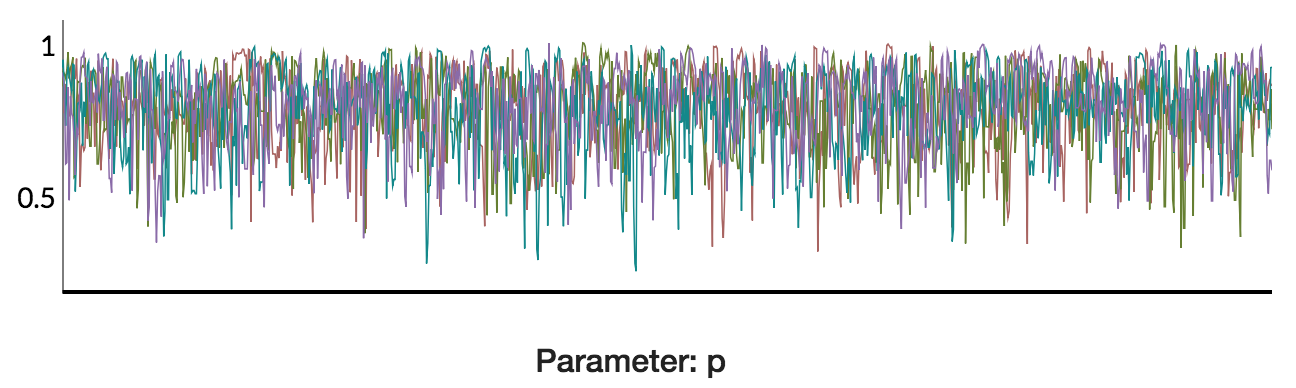
\includegraphics[scale=0.3]{markov_coin.png}
 		\caption{Те самые четыре марковские цепи} 
 	\end{center}
 \end{figure}


С помощью этой диаграммы можно отслеживать пошло ли при генерации что-то не так. 

\todo[inline]{Вставить пример расходящейся цепи}

Среди огромной череды картинок нас прежде всего будут интересовать апостериорные распределения параметра $p$ и прогноза $y_{new}$. Пунктирной линией на картинке обозначена медиана, непрерывной среднее. 

\vspace{1cm}

	\begin{minipage}[H]{0.47\linewidth}
		\begin{center}
			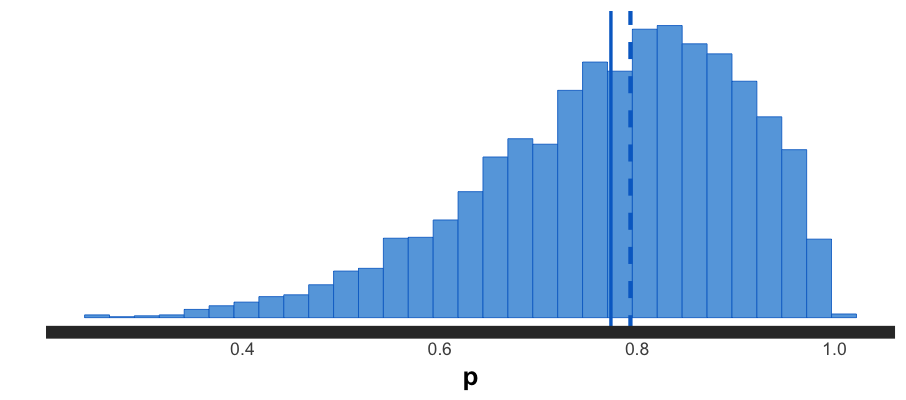
\includegraphics[scale=0.22]{p_coin.png}
		\end{center}
	\end{minipage}
\hfill
	\begin{minipage}[H]{0.47\linewidth}
		\begin{center}
			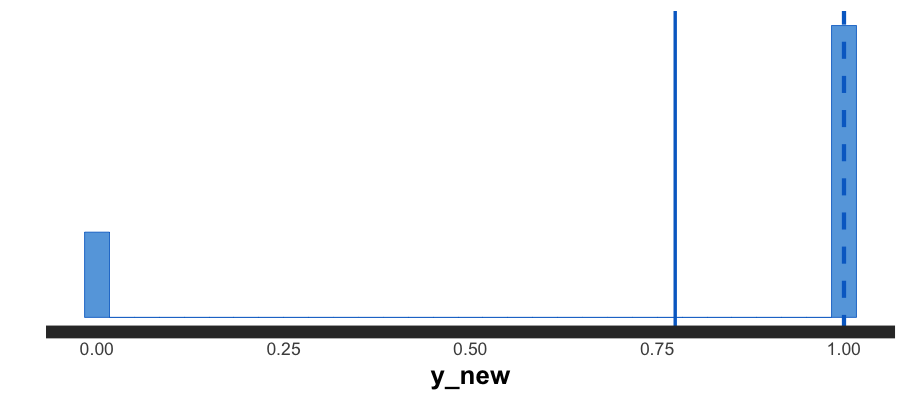
\includegraphics[scale=0.22]{ynew_coin.png}
		\end{center}
	\end{minipage}

 \vspace{0.5cm}
 
 Как и ожидалось, равномерное априорное распределение трансформировалось в горбатое апостериорное.  Априорное распределение довольно легко поменять, отредактировав становский файл, а после заново скомпилировав его. Например, попробуйте заменить равномерное априорное распределение на бэта-распределение. 
 
 На той же веб-страничке во вкладке \textbf{More/Glossary} можно найти описание некоторых метрик, которые расчитываются при сэмплировании. Во вкладке \textbf{Estimate} можно найти готовый генератор латеховских таблиц с результатами сэмплирования. Давайте немного полюбуемся на табличку, а после пробежимся по основным определениям.  Когда мы будем разбираться с устройством MCMC, мы ещё раз поговорим об этих параметрах и способах их расчёта.  
  
\begin{center}
\begin{tabular}{lrrrrrrr}
	\toprule
	Parameter & Rhat & n\_eff & mean & sd & 2.5\% & 50\% & 97.5\% \\ 
	\midrule
	p & 1.0 & 1779 & 0.8 & 0.1 & 0.5 & 0.8 & 1.0 \\ 
	y\_new & 1.0 & 3351 & 0.8 & 0.4 & 0.0 & 1.0 & 1.0 \\ 
	\bottomrule
\end{tabular}
\end{center} 

\begin{itemize}
\item  Мы генерируем апостериорное распределение с помощью марковской цепи. Результат первых итераций нельзя рассматривать как выборку из апостериорного распределения, так как к тому моменту алгоритм ещё не сошёлся. Параметр n\_eff ---  это оценка числа наблюдений, которые мы можем использовать как выборку из апостериорного распределения. Если это число оказалось слишком маленьким, попробуйте увеличить число итераций. 

\item Выборку из апостерирорного распределения мы получим только если марковская цепь сошлась. Промониторить сходимость можно несколькими способами. Как уже говорилось выше, можно посмотреть на картиночки. А можно посмотреть на метрику Rhat. По дефолту STAN генерирует четыре марковских цепочки. Статистика Rhat смотрит на отношение средней межвыборочной дисперсии (посчитали четыре дисперсии и усреднили) к дисперсии, рассчитанной по объединённой большой выборке. Если это отношение близко к единице, цепочки находятся в равновесии. Если они не сходятся к общему распределению, статистика Rhat будет больше единицы. 

\item Ещё одной метрикой мониторинга сходимости является se\_mean.  По всем марковским цепям считаются апостериорные средние. После для них вычисляется средняя квадратическая ошибка. Если хотя бы одна цепь не сошлась, ошибка оказывается высокой. При увеличении числа итераций, при условии сходимости цепей, эта метрика сходится к нулю. 

\todo[inline]{Написать про lp. Это последнее чёрное пятно в протоколе.}

%\item  Последнее чёрное пятно в протоколе это $lp\_\_$.  Предположим, что мы оценили какую-то модель. Возникает вопрос: а подходит ли она под данные? Или всё это ерунда. Как проверить? Идея: давайте сравним наблюдаемые данные с искуственно сгенерированными. Если они не похожи, то модель плохая. 

%Это величина пропорциональна вероятности того, что при нашем апостериорном распределении вывалиться именно наблюдаемая выборка. Конечно же при разных значениях пар
\end{itemize} 

Подведём итоги. STAN позволяет довольно просто, с помощью человеческого языка оценивать разные модели. На выходе мы получаем целое распределение! Вычленив его из нашей модели, мы можем отвечать на разные, интересующие нас вопросы. Например, вот так можно узнать какова вероятность, что $p$ больше $0.5$

\begin{minted}[breaklines,linenos]{R}
p_aposterior = extract(fit)$p
sum(p_aposterior > 0.5)/length(p_aposterior)
\end{minted}

STAN взаимодействует со всем, что движется: R, python, julia, matlab, stata. У него довольно подробная инструкция, логарифм числа страниц в ней чуть больше шестёрки, 

\[ln(pages) \approx 6.36.\]

Даже официальных примеров куча, 

\[ln(examples) \approx 6.04.\] 

 Подгрузить примеры в RStudio можно командой \mintinline{R}|md <- stan_demo()|.  В конце главы читатель с широким кругозором может найти целый пул  источников информации по STAN. 

Давайте напоследок посмотрим на то как меняется апостериорная плотность, когда к нам поступает всё больше и больше новых данных.  Представим себе, что монетка трижды выпала орлом, потом один раз решкой, а потом снова два раза орлом.  

\begin{center}
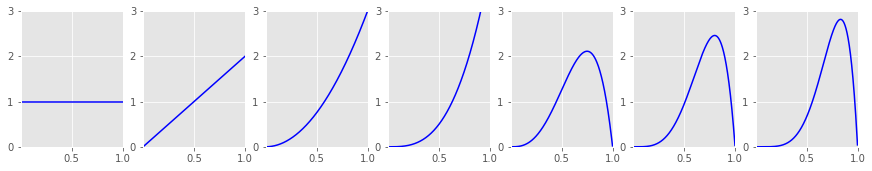
\includegraphics[scale=0.45]{beta_coin_evol.png}
\end{center}

В самом начале мы ничего не знаем о монетке и считаем, что $p$ равномерно распределена на отрезке от нуля до единицы. При поступлении информации о первом орле, наши представления меняются, и вероятностная масса перетекает направо. Следущие два орла укрепляют нашу уверенность в том, что монета неправильная. Первая решка сбивает с нас спесь и распределение наконец становится горбатым.  Следущие два орла сдвигают моду распределения вправо и делают его более вытянутым. 

При каждом пересчёте параметры $\alpha$ и $\beta$ нашего распределения растут, разброс для случайной величины $p$ становится всё меньше, а купол становится всё острее.  Попробуем перейти от монетки к паре более интересных задачек. 

\section{Наивный байесовский классификатор} 

Представим себе следущую ситуацию: мы проснулись утром, заварили себе чаёк, взяли пару печенек и открыли почту, а там куча писем.  Десяток про виагру, десяток про айфон в кредит и ещё двадцаток про онлайн-казино. Получить такое  не очень приятно. Сразу хочется закрыть почту и завести себе сову или голубя. 

Любому почтовому сервису хотелось бы, чтобы пользователь пореже получал спам и не хотел заводить себе почтовое животное.  Для этого был придуман наивный байесовский алгоритм. Машина считает сколько раз слово виагра (и другие слова) встречается в нормальных письмах, а сколько раз в спаме.  На основе этих частот машина по формуле байеса находит вероятность, что письмо является плохим и ежели что, отправляет его в отдельную папку со спамом. 

Классификатор писем на спам и не спам называется байесовским, так как он использует формулу Байеса. Наивным он называется, потому что перед применением мы делаем предположение о том, что вероятности попадания отдельных слов в письмо, не зависят друг от друга. На самом деле это неправда, и это предположение довольно наивно. Отсюда и название --- наивный байес. 

В самом начале главы мы сказали, что перед тем, как описывать математическую модель, полезным бывает представить в голове как именно устроено исследуемое нами явление с вероятностной точки зрения. Отбросим все предрассудки! Мир создал он --- процесс порождения данных, и в случае спама он представляет собой пару мешков. 

\begin{center}
	\definecolor{qqqqff}{rgb}{0.,0.,1.}
	\begin{tikzpicture}
	\node[inner sep=0pt] (russell) at (-2.5,0)
	{
\includegraphics[width=.25\textwidth]{meshok.png}};
	\draw (-3.8,0) node[anchor=north west,scale=1.6] {$SPAM$};
	
	\node[inner sep=0pt] (russell) at (2.5,0)
	{
\includegraphics[width=.25\textwidth]{meshok.png}};
	\draw (1.4,0) node[anchor=north west,scale=1.6] {$HAM$};
	\end{tikzpicture}
\end{center}


В каждом из мешков лежат камешки. На каждом камешке написано некоторое слово. Камешки с одинаковыми словами повторяются какое-то количество раз. В разных мешках разные наборы камешков. Конечно же, слово <<виагра>> есть и в мешке со спамом, и в мешке с нормальными сообщениями, но  в мешке со спамом оно встречается гораздо чаще.  Природа, перед тем как отправить письмо на наш почтовый ящик, генерирует его, доставая камешки из одного из мешков. Сначала она подкидывает неправильную монетку. В зависимости от того, какой стороной она выпала, природа определяется с мешком. Пусть ей посчастливилось выбрать мешок со спамом.  Природа начинает тянуть из этого мешка камешки и выстраивать спамное сообщение. 

\begin{center}
	\definecolor{qqqqff}{rgb}{0.,0.,1.}
	\begin{tikzpicture}
	\node[inner sep=0pt] (russell) at (-2.5,0)
	{
\includegraphics[width=.25\textwidth]{meshok_spam.png}};
	\draw (-3.8,1.1) node[anchor=north west,scale=1.6] {$SPAM$};
	
	\node[inner sep=0pt] (russell) at (2.5,0)
	{
\includegraphics[width=.25\textwidth]{meshok.png}};
	\draw (1.4,0) node[anchor=north west,scale=1.6] {$HAM$};
	\end{tikzpicture}
\end{center}

После сообщение отправляется к нам на почту. Вероятность увидеть конкретное письмо у себя на почте можно найти по формуле полной вероятности: 

\[ \PP(text) = \PP(text \mid spam) \cdot \PP(spam)  + \PP(text \mid ham) \cdot \PP(ham).\] 

Мы можем по размеченной выборке оценить вероятности $\PP(text \mid spam)$ и $ \PP(text \mid ham) $.  У нас есть какое-то письмо $text$, оно состоит из слов $w_1, \ldots, w_n$ и, возможно, является спамом.  Давайте посчитаем как часто конкретное слово встречается в спаме  $n_s$ и поделим это число на общую частоту слова $n_w$, получая при этом вероятность того, что слово всплывёт в спамном сообщении

\[\PP(w \mid spam) = \frac{n_s}{n_w} \qquad  \PP(w \mid ham) = \frac{n_h}{n_w} \]

Перемножив вероятности встретить каждое из слов сообщения в спаме, мы получим вероятность появления этого текста, при условии что оно само является спамом

\[ \PP(text | spam ) = \PP(w_1 \mid spam) \cdot \ldots \cdot \PP(w_n \mid spam).\]

Именно здесь делается наивное предположение о независимости слов в сообщении.  Это неправда. К сожалению, совместную вероятность $\PP(w_1 \ldots w_n \mid spam)$ оценить очень сложно. Для этого нам пришлось бы собрать громадный набор текстов, в который каждая из существующих последовательностей из слов вошла бы по несколько раз. Причём чем больше, тем лучше. Такая задача выглядит нерешаемой. Из-за этого приходится делать наивное предположение, что вероятности вхождения слов в текст --- независимые события. 

Мы научились по выборке оценивать  $ \PP(text | spam ) $.  Когда мы говорим о процедуре порождения текста, мы говорим о прямой задаче. Нас больше интересует обратная задача, состоящая в понимании того, при каких условиях родился текст. Перейти от прямой задачи к обратной помогает формула Байеса. Перевернём игру. 

\begin{multline*}
\PP(spam \mid text)  \propto  \PP(text \mid spam) \cdot \PP(spam) \propto \\ \propto \PP(w_1 \mid spam) \cdot \ldots \cdot \PP(w_n \mid spam) \cdot \PP(spam)
\end{multline*}

Как оценить вероятности $\PP(w_i \mid spam)$ мы обсудили выше. По сути их произведение это ни что иное как функция правдоподобия.  Вероятность $\PP(spam)$ представляет собой априорную вероятность того, что сообщение перед нами является спамом. Если вы ничего не знаете о спаме, можно взять в качестве априорного распределения равномерное. При нём вероятность спама будет равна $0.5$.  Недавние исследования показали, что на сегодняшний день вероятность того, что сообщение, попавшее на почту является спамом, составляет около $0.8$. В принципе, априорно можно быть очень скептическим и проповедовать презумпцию спама, оценивая $\PP(spam)$ очень высоко\footnote{Найти эту не очень радостную статистику можно тут: http://certmag.com/more-than-90-percent-of-e-mails-in-third-quarter-were-spam/}. 

После того, как мы научим классификатор распознавать спам, мы сможем для каждого нового сообщения получить апостериорные вероятности $\PP(spam \mid text)$  и $\PP(ham \mid text)$. В качестве прогноза мы выберем тот класс, вероятность появления для которого больше. Это правило можно записать следующим незатейливым образом

\[ \hat y = \argmax_{y} \PP(text \mid y) \cdot \PP(y). \] 

Переводится как: выбирай тот $y$ для которого апостериорная вероятность максимальна. 

Обучая классификатор (под обучением подразумевается оценка вероятностей для каждого слова и применение формулы Байеса) мы работаем с текстами писем. Вполне возможно, что в одном из новых писем мы встретим какое-то новое слово, которого не оказалось в нашей выборке. Вероятность его появления в спаме будет равна нулю. Итоговая вероятность занулится. Для того, чтобы такого не произошло, нужно будет либо выбросить все неизвестные слова из письма, либо сгладить вероятности, добавив в них дополнительное слагаемое, которое помешает им занулиться
	
	\[ \PP(w \mid spam) = \frac{n_s + a}{n_w + a + b} \qquad \PP(w \mid ham) = \frac{n_s + b}{n_w + a + b}.\]
	
В качестве $a$ и $b$ обычно берут какие-нибудь маленькие числа.  Для сглаживания нужно ввести два числа, чтобы вероятности в сумме по-прежнему давали единицу.  

Попробуем оценить два фильтра: без предубеждений (с априорной вероятностью спама $0.5$) и с предубеждениями (с априорной вероятностью спама $0.8$) и посмотреть какой из них лучше справляется со своими обязанностями.  

В наших руках есть табличка. По строкам в ней отложены письма, по столбцам слова.  В первом столбце стоит вердикт было ли сообщение спамом. Во втором столбце стоит $1$, если слово make встретилось в письме и $0$, если не встретилось, в третьем столбце та же информация приведена по слову adress и так далее (вместо факта вхождения слова в письмо можно было бы собирать количество слов в письме, суть от этого не меняется, но качество работы классификатора улучшается).

\begin{center}
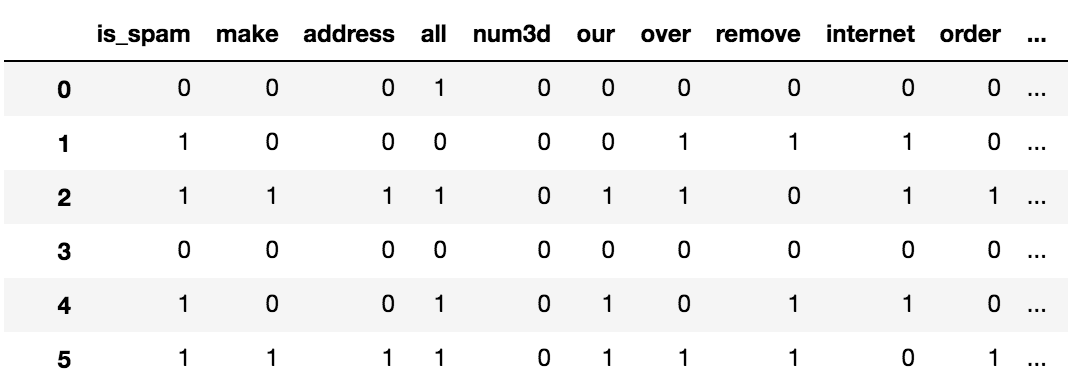
\includegraphics[scale=0.27]{spam_table.png}
\end{center}

Давайте попробуем на этих данных оценить байесовский классификатор. Следущие два абзаца для прошаренного читателя будут очевидными. Разобьём всю выборку на две части: обучающую и тестовую. На обучающей выборку мы будем искать для каждого слова условные частоты. На тестовой выборке мы будем проверять насколько точно работает наш классификатор.  Проверять качество модели на обучающей выборке --- нечестно!  Из-за того, что мы учили частоты на этой выборке, качество модели на ней будет завышено. Она не встретит ничего непредсказуемого. Нам же хотелось бы видеть как модель работает в боевых условиях.  Именно поэтому мы откладываем тестовую выборку. 

Вообще сама по себе ситуация, когда модель вылизывает обучающую выборку, называется переобучением. Тестовая выборка должна помочь нам такую ситуацию отловить. Иногда выборку дробят не на две, а на три части: обучающую, валидационную и тестовую. При таком дроблении на обучающей выборке тренируют модель, на валидационной подбирают гиперпараметры (пример таких гиперпараметров вы найдёте через раздел), а на тестовой проверяют качество модели. 

Дальше мы будем вбивать модель в STAN, оценивать её и получать прогнозы. Чтобы лучше понимать что происходит, попробуйте самостоятельно закодить наивного байеса в R без участия STAN. Это задание мы вынесли в конец главы в отдельное упражнение. К нему есть решение. Имеет смысл попробовать сделать его уже сейчас. Обратите внимание, что для удобства выборка уже разбита на \href{https://raw.githubusercontent.com/FUlyankin/bayes_book/master/itog_scripts/naive_bayes/spam_train.csv}{обучающую} и \href{https://raw.githubusercontent.com/FUlyankin/bayes_book/master/itog_scripts/naive_bayes/spam_test.csv}{тестовую.} 

Сделали? Тогда врываемся в STAN. Создаём файлик \textbf{naive\_bayes.stan} и начинаем его понемногу заполнять. 



\todo[inline]{Возникли проблемы с тем, чтобы нормально задать связь между y и X. Пока без алгоритма на стане. Плак плак плак...}


Качество угадывания оказалось равно $75\%$. Если каждое сообщение обзывать спамом, точность прогноза будет $42\%$. Если каждое сообщение называть хорошим, точность прогноза составит $58\%$. Поздравляю! Наш байесовский классификатор работает существенно лучше константного алгоритма. Можно побороться за качество его работы и расширить выборку из слов и писем. При больших выборках она окажется порядка $99\%$. 

В реальном мире довольно часто оказывается, что интуитивные простые модели работают лучше сложных и навороченных. Перед тем как оценивать какую-нибудь забубенистую нейросеть, попробуйте сначала оценить несколько простых моделей. Возможно, они будут работать хорошо, и их качества вам уже будет хватать. В крайнем случае их можно будет использовать как стартовую точку.  

Первая известная программа, фильтрующая почту с помощью байесовского классификатора появилась в 1996 году.  Примерно года эдак до 2010 все почты оборудовали байесовским классификатором и этого хватало.  Со временем спамеры стали хитрее и научились обходить фильтр Байеса, просто вставляя в конец письма много слов, которые часто фигурируют в хороших письмах. Такой метод обхода получил ироничное название отравление Байеса, а фильтровать спам стали другими алгоритмами. 

В современных спамовых фильтрах  стараются учитывать совместные появления слов.  По большому корпусу текстов смотрят какие слова чаще всего встречаются вместе и добавляют такие устойчивые словосочетания, называемые \indef{биграммами} в модель. Иногда смотрят ещё и триграммы. Также тексты перед построением модели обычно предобрабатывают. Например, выбрасывают нейтральные слова, которые встречаются во всех текстах подряд и не несут никакой информации о его природе.  Обычно такими словами являются союзы, предлоги и тп. Их называют \indef{стоп-словами}. Ещё стараются привести разные формы слова к одной форме. Так слово <<люди>> пытаются привратить в слово <<человек>>, а слово <<предкризисный>> в слово <<кризис>>. Такая процедура называется \indef{нормализацией}. Когда мы будем говорить про вероятностные модели, связанные с порождением текстов, мы подробнее поговорим про все эти методы предобработки. 


\section{Лирическое отступление}

Давайте ликвидируем ещё немного безграмотности. Обычно, когда ты спрашиваешь у человека про то, с помощью какой случайной величины можно замоделировать счётчик (число лайков, число людей в очереди, число букв <<п>> на странице книги), человек отвечает, что для этого идеально подходит распределение Пуассона, которое рождается из распределения Бернулли\footnote{Ну либо говорит <<Ээээээ>>.}. 

Если спросить того же человека о том, с помощью какого распределения можно смоделировать время, которое нужно прождать до появления события (врямя до нового лайка, до нового человека в очереди, до новой поломки станка и тп), то он скажет, что для этого идеально подходит экспоненциальное распределение. 

Выходит, что распределение Пуассона и экспоненциальное распределение как-то связаны. Если того же самого человека спросить как, он почти наверное не ответит. Давайте попробуем ликвидировать этот небольшой пробел в образовании. 

Любую Пуассоновскую случайную величину можно увязать со временем. Например, можно рассматривать число лайков, которые сорвал пост за промежуток времени $t$. Тогда Пуассоновская случайная величина превращается в \indef{простейший поток событий}.  Вероятность того, что за промежуток $t$ наступит $k$ событий будет считаться по формуле 

\[ \PP_t(k) = \frac{e^{-\lambda t} \cdot (\lambda t)^k}{k!}. \]

Простейший поток событий обладает несколькими интересными свойствами: 

\begin{enumerate}
	\item \indef{Стационарность.} Появление $k$ событий на каком-то промежутке зависит только от числа $k$ и от длины этого промежутка. Точка начального отсчёта не имеет значения. 
	\item \indef{Ординарность.} Наступление более одного события этого потока за бесконечно малый промежуток времени является практически невозможным. 
	\item \indef{Отсутствия после действия.}  Вероятность появления $k$ событий на любом промежутке времени не зависит от того сколько событий произошло до этого. 	
\end{enumerate}

Все эти свойства можно довольно легко доказать. Невооруженным взглядом видно, что вероятность зависит только от $k$ и $t$, что характеризует стационарность потока, в формуле не используется никакой информации о том сколько событий наступило до этого, что характеризует свойство отсутствия после действия. Немного поколдовав можно убедиться в ординарности. Можно даже отталкиваясь от этих свойств получить формулу Пуассона.  Мы не будем делать это\footnote{Можно посмотреть как это делается в книге Б.В. Гнеденко <<Курс Теории вероятностей>> на страницах 294-300.} . 

Перейдём к самому интересному. Пусть $T$ это промежуток времени между событиями. Давайте попробуем найти функцию распределения для этой случайной величины. 

Будем делать ровно также, как мы делали это на семинарах по теории вероятностей ... через вероятность. Нас интересует 

\[ F_T(t) = \PP(T \le t).\]

Вероятность $\PP(T \le t)$ можно прочитать, как вероятность возникновения хотябы одного события в течение первых $t$ минут. Вероятность того, что за $t$ минут не возникнет ни одного события можно записать как 

\[1 - F(t) = \PP(T > t).\]

Это логично, если время ожидания $T$ перевалило за $t$, значит ни одного события ещё не наступило. На языке распределения пуассона 

\[\PP(T > t) = \PP_0(t) = e^{-\lambda t}.\] 

Значит 

\[ F_T(t) = 1 - e^{-\lambda t}, \quad t \ge 0.\]

Получилась функция распределения экспоненциальной случайной величины. Прочувствовали связь?  Давайте немного углубим её. Для Распределения Пуассона математическое ожидание составляет $\lambda$. Этот параметр интерпретируется как интенсивность потока событий. Чем он больше, тем больше событий за единицу времени может произойти. 

Для экспоненциального распределения математическое ожидание составляет $\frac{1}{\lambda}$. Чувствуете? Чем больше интенсивность потока событий, тем меньше в среднем времени проходит между ними.  Теперь вы больше знаете о том, как взаимосвязаны между собой Пуассоновская и экспоненциальная случайные величины, и мы можем закончить с лирическим отступлением и перейти к следующему примеру в STAN. 

\section{О Пуассоне и структурных сдвигах} 

Думали, что мы уже закончили бороться со спамом? Нет, всё только начинается.  Давайте проанализируем более интересный пример. Он касается скорости, с которой пользователь отправляет и получает сообщения. 

Все мы пользуемся социальными сетями. Все мы пишем сообщения в некотором режиме. Иногда происходит ужасное, в наш аккаунт вламывается спамер и начинает всем рассылать непристойности. С помощью байесовских методов можно попытаться найти тот момент времени, когда в поведении пользователя произошло неожиданное изменение. Такие изменения в поведении принято называть \indef{структурными сдвигами.}

Сразу же стоит оговориться, что структурный сдвиг байесовские методы то найдут, но не факт, что он происходит именно из-за взлома аккаунта. Возможно, всплеск в сообщениях произошёл по какой-то иной причине.  Мы можем лишь идентифицировать его наличие в данных. Поэтому сразу же предостережём читателя, сказав, что для полноценной борьбы со злоумышленниками придётся строить более сложные модели. Например, с помощью байесовских методов можно понимать в какой момент произошёл структурный сдвиг, а после с помощью накрученного поверх классификатора (любого от логистической регрессии до нейросетки, можно даже байесовского, хватало бы только данных для обучения) можно было бы определять был ли этот структурный сдвиг злокачественным. 

Давайте посмотрим на \href{https://raw.githubusercontent.com/FUlyankin/bayes_book/master/itog_scripts/poisson_shift/message.csv}{следущие данные:}\footnote{Этот пример позаимствован из книги <<Байесовские методы для хакеров>>. Ознакомиться с оригиналом можно по ссылке : \url{ } Там вас ждёт решение части этой же задачки на питоне.}

\begin{center}
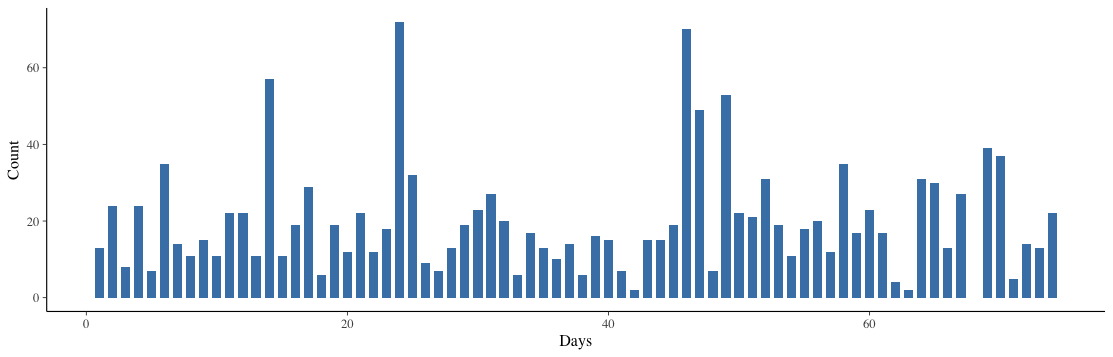
\includegraphics[scale=0.35]{poisson_shift1.png}
\end{center} 

По оси $x$ отложены дни, по оси $y$ количество сообщений, отправленное пользователем в каждый из дней.  Моделировать такие штуки можно распределением Пуассона. Параметр $\lambda$ отражает то, насколько интенсивно отправляются сообщения. Большие значения $\lambda$ присваивают большую вероятность более высоким значениям случайной величины. 

Пусть в некоторый момент времени в поведении пользователя происходят изменения, он начинает писать больше сообщений, чем обычно. Момент, когда произошёл такой структурный сдвиг обозначим буквой $\tau$. После наступления этого момента случайная величина стала стабильно принимать большие значения, значит интенсивность потока сообщений возросла и $\lambda$ увеличилась. Таким образом до момента $\tau$ случайная величина имела распределение Пуассона с одной интенсивностью, после момента $\tau$ интенсивность подскочила. 

\begin{equation*}
X_t \sim \begin{cases}  Poiss(\lambda_1), \text{ если } t < \tau \\  Poiss(\lambda_2), \text{ если } t \ge \tau \end{cases}
\end{equation*}

Если при этом никакого скачка в данных не было, то на выходе мы получим, что значения $\lambda_1$ и $\lambda_2$ будут очень близки, а их апостериорные распределения окажутся очень похожи. 

Итак, у нас есть два параметра $\lambda$. Мы хотели бы оценить их используя процедуру байесовского вывода. Для этого нам нужно выбрать для $\lambda$ априорные распределения. Что мы знаем об этих параметрах? Они могут принимать положительные значения. Скорее всего, их значения сосредоточены в какой-то конкретной области. Можно было бы попробовать использовать в качестве априорного распределения экспоненциальное $\lambda \sim Exp(\alpha)$. 

Однако есть одна проблема. У экспоненциального распределения также есть параметр. Не очень понятно откуда его брать. Он находится как-бы за рамками нашей основной модели. Такие параметры называют \indef{гиперпараметрами.}  Можно поступить с ним несколькими способами: 

\begin{itemize}
\item Придумать, опираясь на свои знания о структурных сдвигах, социальных сетях и сообщениях. Не забудьте быть максимально честным с собой.
\item Ввести в модель ещё один уровень иерархии и сказать, что мы практически ничего про $\alpha$ не знаем, то есть  $\alpha \sim U[0, + \infty]$.
\item На данные смотреть в байесовском подходе до процедуры вывода нельзя. Но давайте поглядим. Оценим $\alpha$ по выборке, как $\frac{1}{\bar x}$, вспомнив о том как именно взаимосвязаны между собой экспоненциальное распределение и распределение Пуассона и будем оценивать оценку гиперпараметра в качестве априорной. Такой способ комбинирования частотной статистики с байесовской более-менее честный, однако не подойдёт для идеалиста. 
\item Можно подсмотреть в данные чуть хитрее. Если наша цель спрогнозировать, то можно раздробить выборку на обучающую и валидационную, а после по решётке перебрать все разумные значения гиперпараметра. В итоге выбрать тот, с которым прогнозы самые крутые. Возможно, это поможет выжать из модели максимум. 
\end{itemize}

Мы попробуем применить второй и третий способы. Модель почти собрана. Осталось обсудить лишь структурный сдвиг $\tau$. Это тоже параметр. Мы не знаем когда он произошёл, поэтому скажем, что $\tau \sim U[0;70]$. Итак, наша модель: 

\begin{equation*}
\begin{aligned}
&X_t \sim \begin{cases}  Poiss(\lambda_1), \text{ если } t < \tau \\  Poiss(\lambda_2), \text{ если } t \ge \tau; \end{cases}\\
&\lambda_1 \sim Exp(\alpha); \\
&\lambda_2 \sim Exp(\alpha); \\
&\tau \sim U[0;70]; \\ 
&\alpha = \frac{1}{\bar x}.\\
\end{aligned}
\end{equation*}

С математической точки зрения у нас получилась редкостная монстрятина. Давайте перебьём её в STAN и посмотрим как он с ней разберётся.  Перед этим найдём по выборке, что $\frac{1}{\bar y} = 0.05$, для того чтобы использовать это знание при моделировании $\lambda$. 

\begin{minted}[breaklines,linenos]{C++}
data{
    int N;    // число наблюдений
    int y[N];  // в веторе y лежит сколько сообщений отправили в какой день
}
parameters{
    real <lower=1, upper=70> tau;  // момент сдвига
    real <lower=0> lambda1;           // интенсивность до сдвига
    real <lower=0> lambda2;          // интенсивность после сдвига
}
model{
    // априорно:
    tau ~ uniform(0, 70); 
    lambda1 ~ exponential(0.05);
    lambda2 ~ exponential(0.05);
    // модель: как наблюдения связаны с параметром
    for (n in 1:N) {
        if(n < tau){
            y[n] ~ poisson(lambda1); 
        }else{
            y[n] ~ poisson(lambda2); 
        }
    }
}
// Чтобы было коректно в последняя строка традиционно пустая
\end{minted}


Оборачиваем всё это дело в R ровно тем же самым кодом, что и в предыдущих случаях: 

\begin{minted}[breaklines,linenos]{R}
model <- stan_model(file = "poisson_shift.stan")
dff <- list(N = length(y), y = y)

# Получаем выборку из апостериорных распределений:
fit <- sampling(model, data = dff,iter = 5000)
fit   # Посмотрим на наш fit 
\end{minted}

Итоговый протокол оценивания модели будет выглядеть как-то так: 

\begin{table}[H]
	\centering
	\begin{tabular}{lrrrrrrr}
		\toprule
		Parameter & Rhat & n\_eff & mean & sd & 2.5\% & 50\% & 97.5\% \\ 
		\midrule
		tau & 1.0 & 1486 & 44.8 & 0.9 & 42.7 & 45.0 & 46.0 \\ 
		lambda1 & 1.0 & 2095 & 17.7 & 0.6 & 16.5 & 17.7 & 19.0 \\ 
		lambda2 & 1.0 & 1945 & 22.7 & 0.9 & 21.0 & 22.7 & 24.5 \\ 
		\bottomrule
	\end{tabular}
\end{table}

Напомним, что байесовский вывод возвращает нам целое распределение. В протоколе можно найти только точечные характеристики этих распределений. Давайте посмотрим как выглядят апостериорные гистограммы: 


\begin{figure}[H]
	\begin{minipage}[H]{0.47\linewidth}
		\begin{center}
			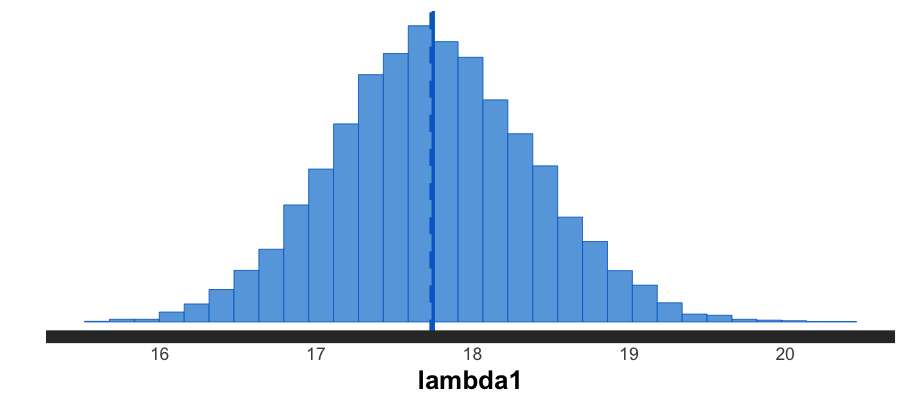
\includegraphics[scale=0.22]{poiss_lambda1.png}
		\end{center}
	\end{minipage}
	\begin{minipage}[H]{0.47\linewidth}
		\begin{center}
			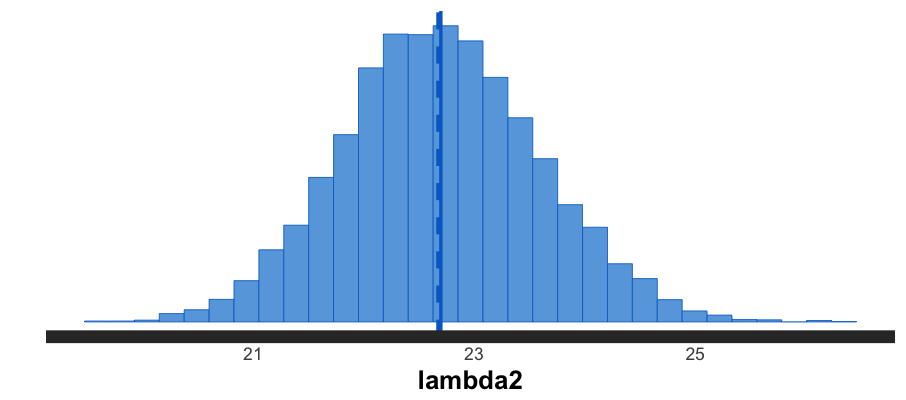
\includegraphics[scale=0.22]{poiss_lambda2.png}
		\end{center}
	\end{minipage}
\begin{minipage}[H]{0.47\linewidth}
	\begin{center}
			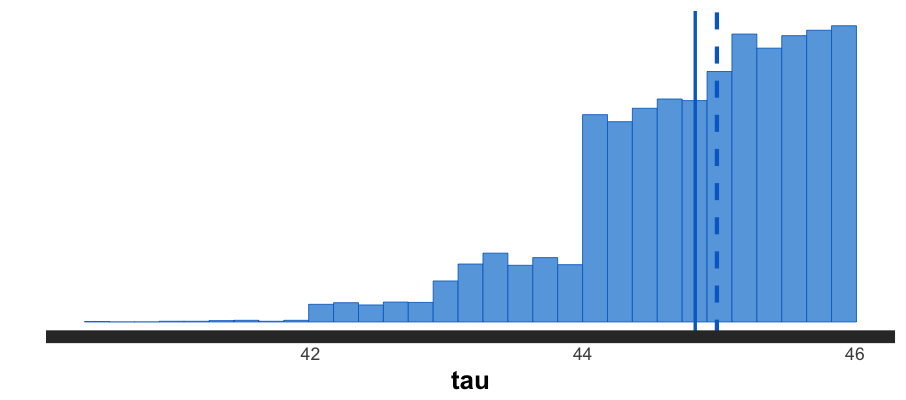
\includegraphics[scale=0.22]{poiss_tau.png}
	\end{center}
\end{minipage}
\end{figure}


Сразу же мы видим неопределённость  в наших оценках. Чем шире распределение, тем меньше наша уверенность в апостериорном результате.  Заметим, что распределения для $\lambda_1$ довольно сильно отличается от распределения для $\lambda_2$. Гистограммы практически не пересекаются. Это говорит о высокой вероятности того, что произошёл структурный сдвиг. 

Обратите внимание, что апостериорные распределение для $\lambda$ вообще не похожи на экспоненциальные. Может возникнуть иллюзия, что они имеют нормальную форму. На самом деле это не так. Обычно апостериорные распределения не имеют какого-то описания через привычные нам станадртные распределения, если конечно это не случай сопряжённых распределений. Если бы мы попытались разрешить сформулированную выше модель аналитически, мы бы упёрлись в интегралы. Использование MCMC позволило избежать этого. 

Распределение для $\tau$ сконцентрировалось в диапазоне от $42$ до $46$. Именно в этот период произошёл структурный сдвиг. В качестве точечной оценки подходит $45$ день. Отметим ещё раз, что если бы никаких изменений не было или если бы изменение было постепенным с течением времени, то распределение для $\tau$ оказалось бы более неоднородным и захватило бы гораздо больший временной диапазон. Мы же видим, что только $4$ дня могут рассматриваться в качестве потенциальных точек структурного изменения.  Давайте нанесём среднее значение случайной величины $X$ до сдвига и после сдвига на нашу картинку с динамикой сообщений. 

\begin{center}
	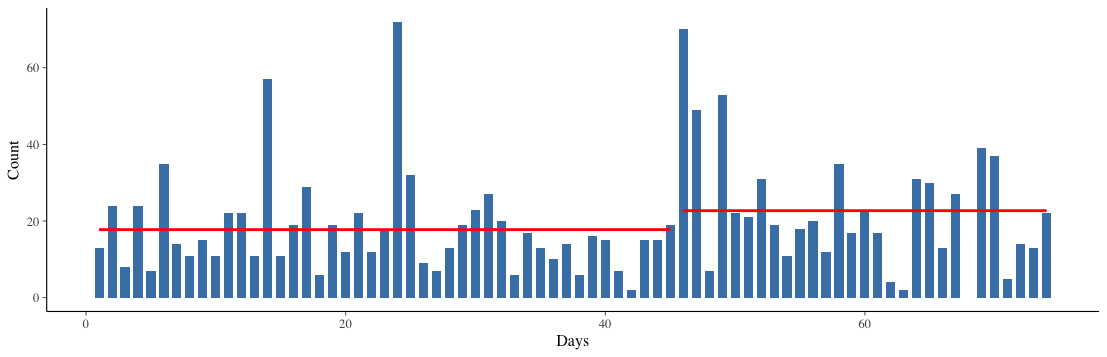
\includegraphics[scale=0.35]{poisson_shift2.png}
\end{center} 

Сдвиг получился не очень большим. В голове рождается мысль, что он связан со статистической погрешностью. Нужна какая-то величина, которая отражала бы нашу степень уверенности в наличии этого сдвига. И у нас такая величина есть. Это $\PP(\lambda_2 > \lambda_1)$. Чтобы сразу же получить её, давайте немного видоизменим модель. Будем говорить, что 

\begin{equation*}
X_t \sim \begin{cases}  Poiss(\lambda), \text{ если } t < \tau, \\  Poiss(\lambda + \varepsilon), \text{ если } t \ge \tau. \end{cases}
\end{equation*}

Тогда мы сразу же после генерации сможем посмотреть по распределению случайной величины $\varepsilon$ насколько велика вероятность структурного сдвига.  Для этого немного подкорректируем наш код в становском файлике:

\begin{minted}[breaklines,linenos]{C++}
parameters{
    real <lower=1, upper=70> tau;  // момент сдвига
    real <lower=0> lambda;
    real  eps;
}
model{
    // априорно:
    tau ~ uniform(0, 70); 
    lambda ~ exponential(0.05);
    eps ~ exponential(0.05);
    // модель: как наблюдения связаны с параметром
    for (n in 1:N) {
        if(n < tau){
            y[n] ~ poisson(lambda);
        }else{
            y[n] ~ poisson(lambda + eps);
        }
    }
}
\end{minted}

Теперь наш структурный сдвиг заложен в $\e$. Апостериорное распределение этого параметра будет выглядеть следущим образом:

\begin{center}
	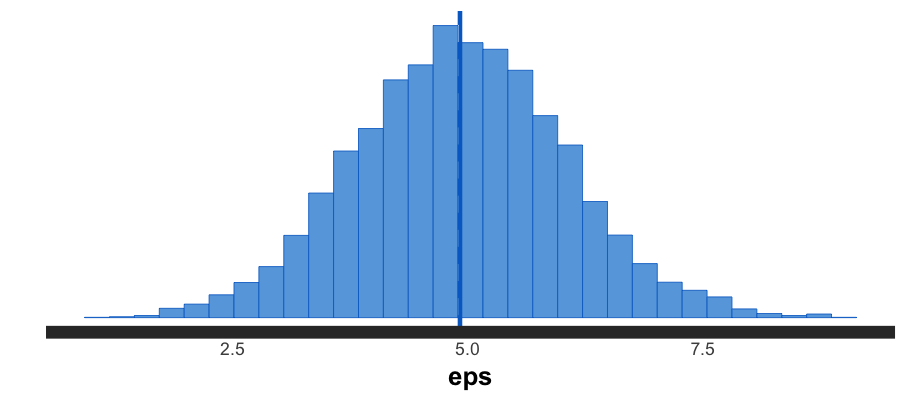
\includegraphics[scale=0.25]{poiss_eps.png}
\end{center}

Вероятностная масса сосредоточена существенно правее нуля. Апостериорно у нас есть все основания верить в него. Вероятность того, что $\e$ больше нуля можно посчитать, вынув из модели апотсериорное распределение. В этом может помочь следущий зверь: 

\begin{minted}{R} 
sum(fit@sim$samples[[1]]$eps > 0)/fit@sim$iter
\end{minted}

Спойлер: $\PP(\varepsilon > 0) = 1 $. Теперь давайте попробуем проделать всё ровно то же самое, но заменим подглядывание в данные для вычисления $\alpha$ на дополнительный уровень в иерархии. 

\begin{equation*}
\begin{aligned}
& X_t \sim \begin{cases}  Poiss(\lambda_1), \text{ если } t < \tau \\  Poiss(\lambda_2), \text{ если } t \ge \tau; \end{cases}\\
&\lambda_1 \sim Exp(\alpha_1); \\
& \lambda_2 \sim Exp(\alpha_2); \\
&\alpha_1 \sim U[0;+\infty]; \\
&\alpha_2 \sim U[0;+\infty]; \\
&\tau \sim U[0;70]. \\ 
\end{aligned}
\end{equation*}


Замоделировать $\alpha_i$ внутри становского кода можно следующим образом: 

\begin{minted}{C++}
alpha1 ~ uniform(0,1000);
\end{minted}

На выходе мы получим ровно такие же распределения для интересующих нас параметров. Распределения для $\alpha_1$ и $\alpha_2$ будут подозрительно похожи на экспоненциальные. В этом любопытный читатель может самостоятельно убедиться, перебив соответствующий код в STAN. 

Пришло время раскрыть правду. На самом деле $45$ день соответствует рождеству. Автор задачи в этот день уехал в другой город к родным, на время расставшись со своей девушкой. Расставание пришлось компенсировать перепиской. Именно из-за этого интенсивность потока сообщений возросла. Мы на этом не прощаемся со структурными сдвигами. Позже мы ещё раз вернёмся к ним, но на этот раз в контексте макроэкономических проблем.  

\todo[inline]{Если эксперименты с вк закончатся успешно, заменть задачу на новую.}


 \subsection{Почиташки про STAN}
 
 
 \begin{itemize}
 	\item \href{https://github.com/stan-dev/stan/releases/download/v2.16.0/stan-reference-2.16.0.pdf}{По ссылке}можно скачать pdf-ку с документацией. 
 	
 	
 	\item  В документации \href{http://mc-stan.org/users/documentation/case-studies.html}{можно найти} большое количество интересных примеров моделирования. Некоторые довольно нетривиальные. 
 \end{itemize}



\section{Ещё задачи}

\begin{problem}
	Немного простых задачек на генерации. Если вы не знаете, какая команда порождает необходимое вам распределение, никто не запрещает подглядеть это \href{https://github.com/stan-dev/stan/releases/download/v2.16.0/stan-reference-2.16.0.pdf}{в документации.} 
	\begin{enumerate}
		\item  Вспомним задачку про Машу и медведей из прошлой главы.  Попробуйте смоделировать её в SNTAN. 
		\item  Попробуйте вбить в STAN задачку про Сашу, Наташу и ресторан ПушкинЪ;
		\item  Вбейте в STAN задачку про подтягунов. Постарайтесь не запутаться в ней; 
		\item  Напишите в STAN код для другой своей любимой задачи из третьей главы. 
	\end{enumerate}

    \begin{sol}
	 По нижеследующим ссылкам можно найти решения всех трёх задачек. 
	 \todo[inline]{Сделать решения} 
	 	\begin{enumerate}
	 	\item  Задачка про Машу. 
	 	\item  Задачка про ресторан. 
	 	\item  Задача о подтягиваниях. 
	 \end{enumerate}	
	\end{sol}
\end{problem}


\begin{problem}
	Придумать упражнение на двумерное нормальное распределение! 
	\begin{sol}
		
	\end{sol}
\end{problem}


\begin{problem}
Помните, что сюжет книги нелинеен? Так вот. В первой главе вы решали задачку на метод максимального правдоподобия. Про наркотики среди студентов. Пришло время решить её ещё разок, но уже используя байесовский подход. Напомню условия задачи.  

Каждый из группы второкурсников, пришедших на пару, подкинул монетку два раза и никому не рассказывал, что у него выпало. В зависимости от того, что выпало на монетках, а также от того пробовал он наркотики или нет, он сказал одну из двух фраз.

\begin{center}
	\begin{tabular}{c|c|c}
		&  выпали два орла   & другая комбинация   \\ \hline
		пробовал наркотики      &   ололо                     &   юпи       \\ \hline
		не пробовал наркотики &	  юпи	                     &   ололо      \\
	\end{tabular}
\end{center}

Таким образом, если человек ололо, либо он курил травку и выпали два орла, либо он не курил травку и выпала другая комбинация. Всегда можно отмазаться. Получается, что при такой форме опроса нет смысла врать, и мы получим из него намного больше информации, чем если бы спрашивали у человека напрямик.  <<Ололо>> сказали $10$ человек, <<юпи>> сказали $4$ человека.

\begin{enumerate}
	\item  Вспомните оценку максимального правдоподобия для доли пробовавших наркотики. 
	\item  C помощью STAN найдите апостериорное распределение доли пробовавших наркотики. 
	\item  Постройте для доли $80\%$ байесовский интервал. Чем этот интервал отличается от доверительного? 
	\item  Исследователь забыл правильную ли он монетку дал ребятам. Пусть $q$ - вероятность орла. Оценить одновременно долю наркоманов и $q$. 
\end{enumerate}

\begin{sol} 
Предположим, что мы вообще ничего не знаем о второкурсниках. В качестве априорного мнения о доле наркоманов возьмём равномерное распределение. 

\[ p \sim U[0;1]\]

На первом этапе все студенты подбрасывают монетку. На ней выпадает одна из заданных комбинаций. На втором этапе природа подбрасывает свою монетку и либо подсаживает студента на наркотики, либо оставляет его в покое\footnote{Реальный мир очень суров.}. 

\end{sol} 	
\end{problem}

\begin{problem}
Самостоятельно на своём любимом языке программирования реализуйте наивного байеса. Используйте для оценивания модели данные из главы. Сравните результаты оценивания с тем, что мы выше получили в STAN.

\begin{sol} 

Скорее всего отважный читатель ринулся со всей своей прытью писать два вложенных друг в друга цикла. Один по словам бегает, другой вхождения считает. Это конечно мило, но можно проще.  Мы будем делать это разными векторными командами! R --- векторный язык программирования. Если какая-то команда вам сходу непонятна, попробуйте применить её отдельно от всего. 

\begin{minted}[breaklines,linenos]{R}
df_train <- read.csv("spam_train.csv")   # подгрузили тренировочную выборку
df_test <- read.csv("spam_test.csv")     # подгрузили тестовую выборку 

n_col = ncol(df_train)   # число столбцов
n_row = nrow(df_train)   # число наблюдений
p_spam = 0.5             # априорная вероятность спама 

# сделали срез по всем сообщениям со спамом и нашли сумму по столбцам
words_spam_freq <- colSums(df_train[df_train[,1] == 1,])

# избавились от столбца с ответами и поделили на число спамных строк
words_spam_freq <- words_spam_freq[2:n_col]/sum(df_train[,1] == 1)

# сделали то же самое с неспамными словами 
words_ham_freq <- colSums(df_train[df_train[,1] == 0,])
words_ham_freq <- words_ham_freq[2:n_col]/sum(df_train[,1] == 0)
\end{minted}

Сейчас в листе $words\_spam\_freq$ лежат $\PP(w_i \mid spam)$.  Лист это структура,  к которой мы можем обращаться по именам столбцов через квадратные скобки. Кусок кода выше отвечает за обучение модели. Мы оценили для каждого слова вероятность встретиться в спамном сообщении. При желании можно завернуть этот код в функцию и как-нибудь красиво назвать. 

Второй частью кода будет применение полученных частот к тестовой выборке.  Для первого наблюдения из тестовой выборки мы можем подсчитать спамность следующим образом: 

\todo[inline]{сделать нормальные формулы!} 

\begin{minted}[breaklines,linenos]{R}
names(df_test[1,])[1]   # выдаст имя первой колонки, то есть слово,  которому соотвествуют частоты в столбце

# выдаст P(w_i | spam) для этого слова 
words_freq[names(df_test[1,,2:n_col])[1]]  

# найдём P(text | spam)*P(spam)
prod(words_freq[names(df_test[,2:n_col])[df_test[1,2:n_col] > 0]])*p_spam

# найдём P(text | ham)*P(ham)
prod(words_ham_freq[names(df_test[,2:n_col])[df_test[1,2:n_col] > 0]])*(1 -p_spam)
\end{minted}

Обратите внимание, что мы при поиске апостериорной вероятности, пренебрегли константой.  Для того, чтобы сделать прогноз нам остаётся сравнить две, полученные на выходе вероятности между собой и определиться с тем, что из себя представляет сообщение. 

\begin{minted}[breaklines,linenos]{R}
# Сделаем прогнозы по всей тестовой выборке
forecasts = c()

for(i in 1: nrow(df_test)){
    spam = prod(words_freq[names(df_test[,2:n_col])[df_test[i,2:n_col] > 0]])*p_spam
    ham = prod(words_ham_freq[names(df_test[,2:n_col])[df_test[i,2:n_col] > 0]])*(1 -p_spam)
    if(spam > ham){
        forecasts = append(forecasts,1)
    }else{
        forecasts = append(forecasts,0)
    }
}

# Посмотрим как часто мы угадываем, где в письмах есть спам
sum(df_test[,1] == forecasts)/length(forecasts)
\end{minted}

Качество угадывания оказалось равно $75\%$. Если каждое сообщение обзывать спамом, точность прогноза будет $42\%$. Если каждое сообщение называть хорошим, точность прогноза составит $58\%$. Поздравляю! Наш байесовский классификатор работает существенно лучше наивного алгоритма. 

Разобрались с наивным байесом? Контрольный вопрос! Предположим, что у нас есть $k$ классов. Наблюдения распределены по ним неравномерно.  Апостериорная вероятность выпадения каждого класса составляет $\PP(y \mid x) = \frac{1}{k}$.  Какой класс в таком случае будет выдавать байесовсий классификатор для произвольного $x$? 

Внимание, ответ: наибольший. 
\end{sol} 
\end{problem} 

%\begin{problem}
%	Рассмотрим данные по количеству происшествий на английских шахтах. Предположим, что до момента $b$ включительно количество происшествий за год имеет пуассоновское распределение с параметром $\lambda_1$, а после момента $b$ — пуассоновское с параметром $\lambda_2$.
%	
%	Всего есть данные за $T$ дней. Предположим, что априорно $b$ равновероятно принимает значения от 1 до $T$, а $\lambda_i \sim IG(rate = 3, shape = 4)$.
%	
%	Фактические данные по количеству происшествий за год рассчитайте исходя из дат происшествий по ссылке \url{http://people.reed.edu/~jones/141/Coal.html}.
%	
%	С помощью STAN:
%	\begin{enumerate}
%		\item Постройте выборку из апостериорного распределения $\lambda_1$, $\lambda_2$, $b$.
%		\item Какой год наиболее вероятно был годом структурного сдвига?
%		\item Постройте прогноз распределения количества аварий на шахтах на следующий год.
%	\end{enumerate}
%	\begin{sol}
%	\end{sol}
%\end{problem}



\begin{problem}

28 января 1986 года двадцать пятый полёт программы космических шаттлов США закончился катастрофой\footnote{Ещё одна задача, взятая из <<Байесовских методов для хакеров>>. }. Один из ракетных ускорителей шаттла <<Челленджер>> взорвался вскоре после взлёта, в результате чего погибли все семь членов экипажа. Президентская комиссия по авиационным происшествиям пришла к выводу, что взрыв был вызван отказом уплотнительного кольца в полевом стыке ракеты-носителя. Кольцо отказала в силу неправильной конструкции, которая сделала уплотнительное кольцо слишком чувствительным к ряду факторов. В том числе к температуре наружного воздуха.

Из предыдущих $24$ рейсов были доступны данные о сбоях $23$ уплотнительных колец (в течение одного из рейсов кольцо потеряли в море).  Эти данные обсуждались вечером накануне трагедии. К сожалению,  важными считались только данные, соответствующие $7$ рейсам, на которых произошло повреждение. Они не показывали очевидной тенденции. Температура оценивается в градусах по Фарингейту. Данные представлены в таблице.

\todo[inline]{скрин таблички с данными }

Итак, вероятность катастрофы зависит от температуры. Обычно, в моделях, где необходимо предсказать вероятность бинарного события, используется сигмоида: 

\[ \PP(t) = \frac{1}{1 + e^{\alpha + \beta t}}.\]

Параметр $\beta$ отвечает за то насколько резко сигмоида перетекает из нулевого состояния в первое. Параметр $\alpha$ отвечает за сдвиг. 

\begin{center}
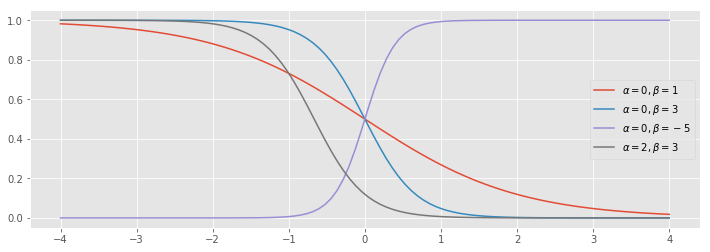
\includegraphics[scale=0.5]{sigmoida.png}
\end{center}

Поначалу вероятность возникновения дефекта довольно низка. По мере изменения температуры она увеличивается. Сначала постепенно, по достижении некоторого критического уровня в вероятности происходит резкий подскок и мы по $S$-образной кривой переходим в новое состояние\footnote{Такая ситуация характерна для многих задач, связанных с классификацией. Например, если мы исследуем зависимость наличия у семьи автомобиля от стоимости дохода, мы понимаем, что поначалу вероятность покупки машины растёт медленно. Как только доход достигает критического уровня, происходит резкий рост вероятности.}. Наша задача оценить как именно происходит этот переход в новое состояние. С помощью STAN: 

\begin{enumerate} 
	\item Найдите апостериорное распределение для параметров $\alpha$ и $\beta$.  Априорно предположите, что $\alpha \sim N(0, 0.001)$,  $\beta \sim N(0, 0.001)$. То есть априорно вероятность катастрофы очень слабо зависит от температуры.
	
	\item Какова вероятность того, что $\alpha$ меньше нуля? Какова вероятность, что $\beta$ меньше нуля? 
	
	\item Представим, что вечером накануне катастрофы вы попали на совещание. Прогноз погоды сообщает, что при завтрашнем запуске температура составит $30$ градусов по Фарингейту. Постройте апостериорное распределение вероятности катастрофы, при этом условии. Постройте для этой вероятности $HPD$. 
	
	\item Вопрос про качество модели. 
	
	\todo[inline]{Добавить про качество модели в текст про структурные сдвиги}
\end{enumerate}
	\begin{sol} 
	Вбиваем в STAN нашу модель. 
	
\begin{minted}[breaklines,linenos]{C++}


\end{minted}
		
		
		
		
	Отметить, что у апостериорных распределений два горба 

	Пояснить за логистическую регрессию 
		
	\end{sol} 
\end{problem}


\begin{problem}
	В группе мемы про машинное обучение для взрослых мужиков постят мемы про машинное обучение для взрослых мужиков. Взрослые мужики смотрят мемы про машинное обучение, лайкают их, комментируют и репостят. В итоге рождается табличка со статистикой.
	
	Предположим, что просмотры, лайки, число комментариев и репосты имеют распределение Пуассона, $X_i \sim Poiss(\lambda)$. Также будем предполагать, что число лайков (и других показателей) на текущем посте не зависит от числа лайков на других постах.
	
	\begin{enumerate}
		\item  ZERO INFLATED MODEL для репостов и лайков 
		\item  HPD для них 
		\item  в какой из ситуаций $p$ нулевые и  тп
		\item  для репостов и для лайков геометрические распределения до первой неудачи, какие из моделей лучше
	\end{enumerate}

	\begin{sol} 
		
	\end{sol} 
\end{problem}


\begin{problem}
	Что-нибудь про шары и гипергеометрическое распределение 
	\begin{sol} 
		
	\end{sol} 
\end{problem}


\begin{problem}
	байесовская оптимизация самостоятельно в R какой-нибудь функции 
	\begin{sol} 
		
	\end{sol} 
\end{problem}


 \begin{problem}
 	
 	\begin{sol} 
 		
 	\end{sol} 
 \end{problem}

\todo[inline]{Задачка на карму, просто подумать}

% \Closesolutionfile{solution_file}
% \input{solutions1}

\end{document}



